\clearpage
\section{Reprezentace znalostí}
Pro řešení prakticky každého reálného problému je potřeba mít k dispozici nějaké znalosti minimálně z oblasti, ve které se problém nachází.
Při řešení problémů pomocí automatický počítačových metod a metod umělé inteligence je pak nutné ještě navíc
mít nějaký způsob, jak tyto znalosti zapsat a uchovat, jak s nimi manipulovat a provádět na nich operace a algoritmy.

Znalost je možné chápat jako nějakou informaci, která popisuje určitý fakt, nebo \enquote{pravdu o světě}.
Jejich vyjádření v nějakém konkrétní podobě, neboli \emph{formalismu}, je potom označováno jako \emph{reprezentace znalostí}.
Tato formální vyjádření by měla umožňovat provádět se znalostmi potřebné operace k vyřešení daného problému.~\cite{prepreze_znal}

Nové znalosti je možné získat v základu dvěma způsoby.
Prvním z nich je pozorování objektů a jevů, což je označováno jako přímé získávání znalostí.
Druhou metodou, která označována jako nepřímá, je odvození nových znalostí z těch, které jsou již známé.~\cite{prepreze_znal}

\subsection{Dělení reprezentace znalostí}
Podle učebního textu~\cite{prepreze_znal} je možné metody reprezentace znalostí rozdělit do několika kategorií.
Schématické znázornění tohoto dělení je na Obrázku~\ref{fig:schema_repreznalosti}.
\begin{figure}[ht!]
	\centering
	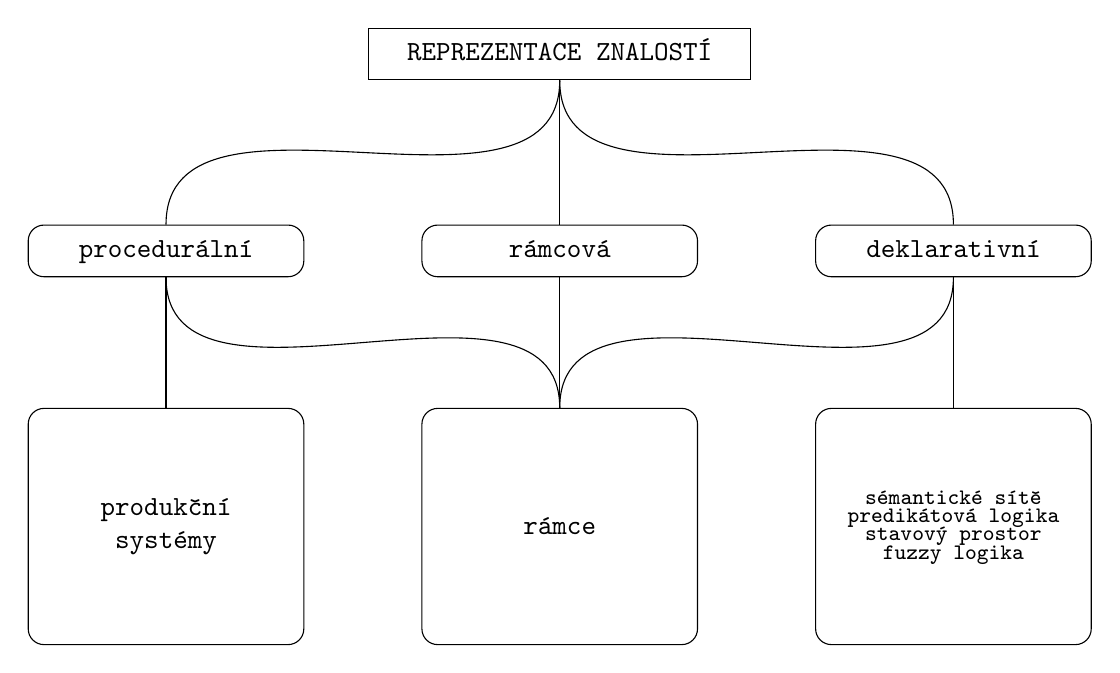
\begin{tikzpicture}
		\node[draw] (main) at (0, 0) {\strut\texttt{\phantom{ll}REPREZENTACE ZNALOSTÍ\phantom{ll}}};
		\node[draw,minimum width=3.5cm, rounded corners=2mm] (procedur) at (-5, -2.5) {\strut \texttt{procedurální}};
		\node[draw,minimum width=3.5cm, rounded corners=2mm] (dekl) at (5, -2.5) {\strut \texttt{deklarativní}};
		\node[draw,minimum width=3.5cm, rounded corners=2mm] (rámc) at (0, -2.5) {\strut \texttt{rámcová}};
		\node[draw,minimum width=3.5cm, minimum height=3cm, rounded corners=2mm] (prodsys) at (-5, -6) {\parbox{3cm}{\centering\texttt{produkční\\systémy}}};
		\node[draw,minimum width=3.5cm, minimum height=3cm, rounded corners=2mm] (mid) at (5, -6)
		{
			\footnotesize
			\begin{tabular}{c}
				\texttt{sémantické sítě}    \\[-1mm]
				\texttt{predikátová logika} \\[-1mm]
				\texttt{stavový prostor}    \\[-1mm]
				\texttt{fuzzy logika}
			\end{tabular}};
		\node[draw,minimum width=3.5cm, minimum height=3cm, rounded corners=2mm] (ramce) at (0, -6) {\texttt{rámce}};
		\draw[-] (main.south) to[out=-90, in=90] (procedur.north);
		\draw[-] (main.south) to[out=-90, in=90] (dekl.north);
		\draw[-] (main.south) to[out=-90, in=90] (rámc.north);
		\draw[-] (procedur.south) to[out=-90, in=90] (prodsys.north);
		\draw[-] (procedur.south) to[out=-90, in=90] (ramce.north);
		\draw[-] (rámc.south) to[out=-90, in=90] (ramce.north);
		\draw[-] (dekl.south) to[out=-90, in=90] (mid.north);
		\draw[-] (dekl.south) to[out=-90, in=90] (ramce.north);
	\end{tikzpicture}
	\caption{Schéma dělení metod reprezentace znalostí~\cite{prepreze_znal}}\label{fig:schema_repreznalosti}
\end{figure}

Deklarativní přístup je založený na vyjádření různých znalostí ve formě \emph{poznatků}, množinou konkrétních a navzájem nezávislých faktů.
S těmito fakty je pak možné manipulovat pomocí takzvaných \emph{procedur}, někdy označovaných jako tvrzení.
Mezi deklarativní metody se také řadí různé přístupy založené na matematice a logice, na algebře, relačních strukturách.
Mezi deklarativní metody se řadí \emph{sémantické sítě}, které znalosti reprezentují jako entity či objekty
relací, které mezi těmito objekty popisují jejich vztahy.
Dalším deklarativním typem reprezentace znalostí jsou \emph{stavové prostory},
které popisují řešený problém jako množinu možných stavů, ve kterých se daný problém může nacházet.
Mezi další formy reprezentace znalostí deklarativní povahy se řadí různé druhy logiky,
jako jsou \emph{predikátová logika} a \emph{fuzzy logika}.~\cite{prepreze_znal}

Procedurální metody reprezentace znalostí zahrnují produkční systémy.
To jsou systémy navržené tak, že pomocí předem dané množiny pravidel, které se označují jako produkční pravidla,
se snaží dosáhnout nějakého stanoveného cíle a vyřešení určitého problému.~\cite{prepreze_znal}

Poslední skupina, označená jako rámcová metoda reprezentace znalostí, představuje kombinaci obou předchozích přístupů.
Rámce jsou struktury, které popisují různé objekty podle předem dané formy a v průběhu řešení
problému se doplňují konkrétní hodnoty k daným vlastnostem.~\cite{prepreze_znal}

Schématická ukázka sémantické sítě využívající rámce je na Obrázku~\ref{fig:frames_net}.
\begin{figure}[ht!]
	\centering
	\begin{tikzpicture}
		\node[inner sep=0pt] (n) at (0, 0) {
			\begin{tabular}{|l|l|}
				\hline
				\emph{Slot}           & \emph{Value}                   \\
				\hline
				\texttt{INSTANCE-OF}: & \texttt{(DOG, PET)}            \\
				Name:                 & \enquote{Fido}                 \\
				Color:                & \texttt{(BROWN)}               \\
				Father:               & \texttt{(BOWSER)}              \\
				Mother:               & \texttt{(WEENIE)}              \\
				Owner:                & \texttt{(MR.-SMITH)}           \\
				% Cost:                 & \ \$12.95                      \\
				Has-as-ears:          & \texttt{(LEFT-EAR, RIGHT-EAR)} \\
				Number-of-ears:       & \texttt{(2)}                   \\
				\hline
			\end{tabular}
		};

		\node[draw=none] (n1) at (8, 0) {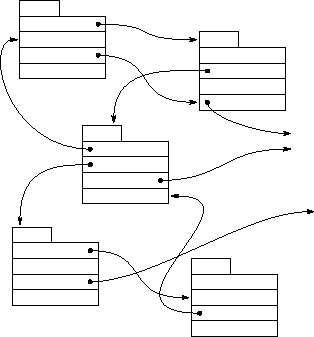
\includegraphics{./src/imgs/frames.pdf}};

		\node[draw, anchor=south west] at ($(n.north west) + (0, -0.5pt)$) {\texttt{(FIDO)}};
	\end{tikzpicture}
	\caption{Ukázka rámce pro individuálního psa (vlevo) a schématické znázornění propojení více rámců (vpravo), převzato z~\cite{semantic-nets-LEHMANN19921}}\label{fig:frames_net}
\end{figure}

\newpage
\subsection{Sémantické sítě}
Sémantické sítě reprezentují znalosti pomocí grafových struktur složených z uzlů a hran.
Uzly představují koncepty či objekty a hrany reprezentují relace mezi těmito jednotkami.
Ukázka jednoduché sémantické sítě je na Obrázku~\ref{fig:semantic_net_example}.

\begin{figure}[H]
	\centering
	\begin{tikzpicture}
		\node[draw, ellipse, minimum width=1.5cm, minimum height=1cm] (dog) at (0,0) {\texttt{pes}};
		\node[draw, ellipse, minimum width=2cm, minimum height=1cm] (sq) at (5,0) {\texttt{kočka}};
		\node[draw, ellipse, minimum width=2cm, minimum height=1cm] (tree) at (2,3) {\texttt{strom}};
		\node[draw, ellipse, minimum width=2cm, minimum height=1cm] (mush) at (5.5,3) {\texttt{kámen}};
		\node[draw, ellipse, minimum width=2cm, minimum height=1cm] (animal) at ($0.5*(dog) + 0.5*(sq) + (0, -2)$) {\texttt{zvíře}};
		\draw[-Stealth, bend left=25] (dog) to node[midway, above] {\footnotesize \texttt{běží za}} (sq);
		\draw[-Stealth] (dog) to node[midway, above] {\footnotesize \texttt{větší než}} (sq);
		\draw[-Stealth, bend left=25] (sq) to node[midway, above] {\footnotesize \texttt{utíká před}} (dog);
		\draw[-Stealth] (sq) -- node[midway, above, sloped] {\footnotesize \texttt{šplhá na}} (tree);
		\draw[-Stealth] (mush) -- node[midway, above, sloped] {\footnotesize \texttt{je pod}} (tree);
		\draw[-Stealth, bend left=30] (mush) -- node[midway, above, sloped] {\footnotesize \texttt{větší než}} (sq);
		\draw[-Stealth] (dog) to node[midway, above, sloped] {\footnotesize \texttt{je pod}} (tree);
		\draw[-Stealth, bend right=30] (dog) to node[midway, above, sloped] {\footnotesize \texttt{je}} (animal);
		\draw[-Stealth, bend left=30] (sq) to node[midway, above, sloped] {\footnotesize \texttt{je}} (animal);
	\end{tikzpicture}
	\caption{Ukázka jednoduché sémantické sítě}\label{fig:semantic_net_example}
\end{figure}

Sémantické sítě umožňují použít různé metody z teorie grafů, logiky a matematiky pro práce s uloženými znalostmi,
jejich analýzu a případně i odpovídání otázek či indukci nových znalostí.
Sémantické sítě se používají v oblastech umělé inteligence pro porozumění jazyku, deduktivní databáze, vyhledávání dokumentů
v databázi, expertní systémy a další.~\cite{semantic-nets-LEHMANN19921}

Sémantické sítě je možné realizovat také s využitím rámců (angl.~frames) pro jednotlivé uzly.
Rámec je chápán jako abstraktní popis nějakého objektu, která má pojmenované \emph{sloty}, které popisují nějaké explicitní vlastnosti.
Tyto rámce mohou být navzájem propojené a odkazovat se na sebe navzájem, čímž tvoří strukturu orientovaného grafu.
Některé implementace také poskytují možnost dynamického zjišťování hodnot pro jednotlivé sloty pomocí procedurálních metod,
což umožňuje zachytit komplexní chování a inferenci.~\cite{semantic-nets-LEHMANN19921}

Podle~\cite{semantic-nets-LEHMANN19921} je možné rozdělit vazby (hrany) v sémantických sítích do několika skupin.
V~relačních grafech, kde hrany popisují relace mezi objekty, tak se označují jako \emph{deskriptivní} nebo \emph{asertivní}.
Oproti \emph{strukturálním}, \emph{definičním} nebo \emph{inferenčním} vazbám, které slouží k zachycení hierarchické struktury objektů,
popisují vyšší abstrakce, kategorie a~dědičnost.~\cite{semantic-nets-LEHMANN19921}

Aby bylo možné pomocí sémantických sítí zachytit i principy logiky, jako jsou:
\begin{itemize}
	\item negace (např.~\enquote{kámen NENÍ zvíře}),
	\item disjunkce (např.~\enquote{osoba narozená v Británii NEBO potomek Brita}),
	\item existenční kvantifikátory (např.~\enquote{VŠECHNY cesty vedou do Říma}),
\end{itemize}
a další komplexnější vztahy, je možné sémantické sítě rozšířit o další typy vazeb (např.~IS-NOT-A) i celé strukturální koncepty,
jako je rozdělení sítě do \emph{prostorů}, které se mohou překrývat jako Vennovy diagramy, což umožňuje vyjádřit složitější logické operace.
Dalším typem rozšíření, který se vyskytuje v \emph{konceptuálních grafech}, je použití \emph{vnořených kontextů},
jejichž principem je využití metod logiky pro vyjádření složitějších operací skrze zapouzdření (angl.~encapsulation) primitivních operací.~\cite{semantic-nets-LEHMANN19921}

\subsection{Ontologie}
Samotná forma reprezentace znalostí a způsob práce s nimi je pouze částí problematiky sémantických sítí,
druhou otázkou, kterou je potřeba řešit, je samotný obsah neboli \enquote{co reprezentovat}.
Tímto problémem se zabývá \emph{ontologie}, která zahrnuje formální označení, strukturu a definice jednotlivých kategorií,
vlastností, relací a samotných dat, které je potřeba reprezentovat.

Svátek~\cite{onto_svatek} uvádí, že cílem ontologie je podpora porozumění mezi lidmi, zejména pak experty v určité oblasti,
podpora komunikace mezi počítačovými systémy a usnadnění návrhu aplikací se znalostním zaměřením.

Rozdělení ontologií do typů či kategorií lze podle~\cite{onto_svatek} dělat podle různých kritérií:
\begin{itemize}
	\item \emph{Dělení podle historického vývoje}:\\
	      V důsledku historického vývoje lze ontologie rozdělit na \emph{terminologické} či \emph{lexikální}, které se zaměřují
	      na textové zdroje a lze je považovat za pokročilé slovníky, poté \emph{informační ontologie}, které jsou spojené s databázovými systémy a schématy
	      a \emph{znalostní ontologie}, které jsou spojené s oblastí umělé inteligence a reprezentace znalostí.
	\item \emph{Dělení podle míry formalizace}:\\
	      Existují typy ontologií, které nejsou celé striktně formalizované a například používají přirozený jazyk pro vysvětlení pojmů.
	      Pak ale také existují striktně formalizované ontologie, které využívají formální jazyky.
	      Podle~\cite{onto_svatek} však většina formálních ontologií obsahuje do nějaké míry i neformální ontologie.
	\item \emph{Dělení podle obsahu}:\\
	      Hlavní typy ontologií podle jejich obsahu jsou doménové, generické, úlohové a~aplikační.
	      Svátek~\cite{onto_svatek} uvádí, že tento způsob dělení je \enquote{tradiční}, avšak s různými variantami, podle konkrétního autora.
\end{itemize}

Struktura ontologií obecně sestává ze \emph{tříd}, \emph{individuí}, \emph{relací}, \emph{pravidel} a \emph{hodnot}.
Třídy odpovídají množinám objektům, někdy jsou také označované jako \emph{kategorie} nebo \emph{koncepty}.
Individua jsou v ontologiích označení pro konkrétní objekty, většinou reprezentující nějaké objekty v reálném světě.
Mezi objekty je možné vytvořit \emph{relace}, které popisují nějaké vazby mezi objekty, či mohou popisovat jejich vlastnosti.
Pravidla, někdy označovaná jako \emph{axiomy}, slouží v ontologických jazycích pro vyjádření logických formulí, jako je ekvivalence tříd, nebo jejich disjunktnost.~\cite{onto_svatek}

Existuje řada různých přístupů a realizací~\cite{semantic-nets-LEHMANN19921}, příkladem může být projekt \emph{Cyc}~\cite{cyc}, jehož cílem je poskytnout ontologii pro reálný svět.
Jiným příkladem může být J. L. Jolleyův \emph{Holotheme}~\cite{jolley1971holotheme}, který se také snaží klasifikovat cokoli,
ovšem v rámci jednoho schématu založeného na strukturální komplexitě.
Dalším příkladem je \emph{Wordtree}~\cite{burger1984wordtree}, který představuje pokus o definici významů slov pomocí kombinování primitivních konceptů a významů.

Jedním z ontologických jazyků je \emph{RDF Schema}~\cite{rdf-schema},
které patří k \emph{Resource Description Framework (RDF)}~\cite{rdf} standardu pod skupinou W3C\footnote{https://www.w3.org/}.
RDF je datový model, který byl navržený pro Web, se zaměřením na kompatibilitu dat a schopnost jejich sloučení.
Je založený na syntaxi značkovacího jazyka XML a hojně využívá URL adresy.
